\thispagestyle{toanhocvadoisongnone}
\pagestyle{toanhocvadoisong}
\everymath{\color{toanhocdoisong}}
\graphicspath{{../toanhocdoisong/pic2/}}
\blfootnote{$^1$\color{toanhocdoisong}Phó Giám đốc phụ trách,
	Sở Thông tin và Truyền thông Hà Nội; Thành viên Tổ công tác giúp việc Uỷ Ban Quốc gia về Chuyển đổi số.}
\begingroup
\AddToShipoutPicture*{\put(0,616){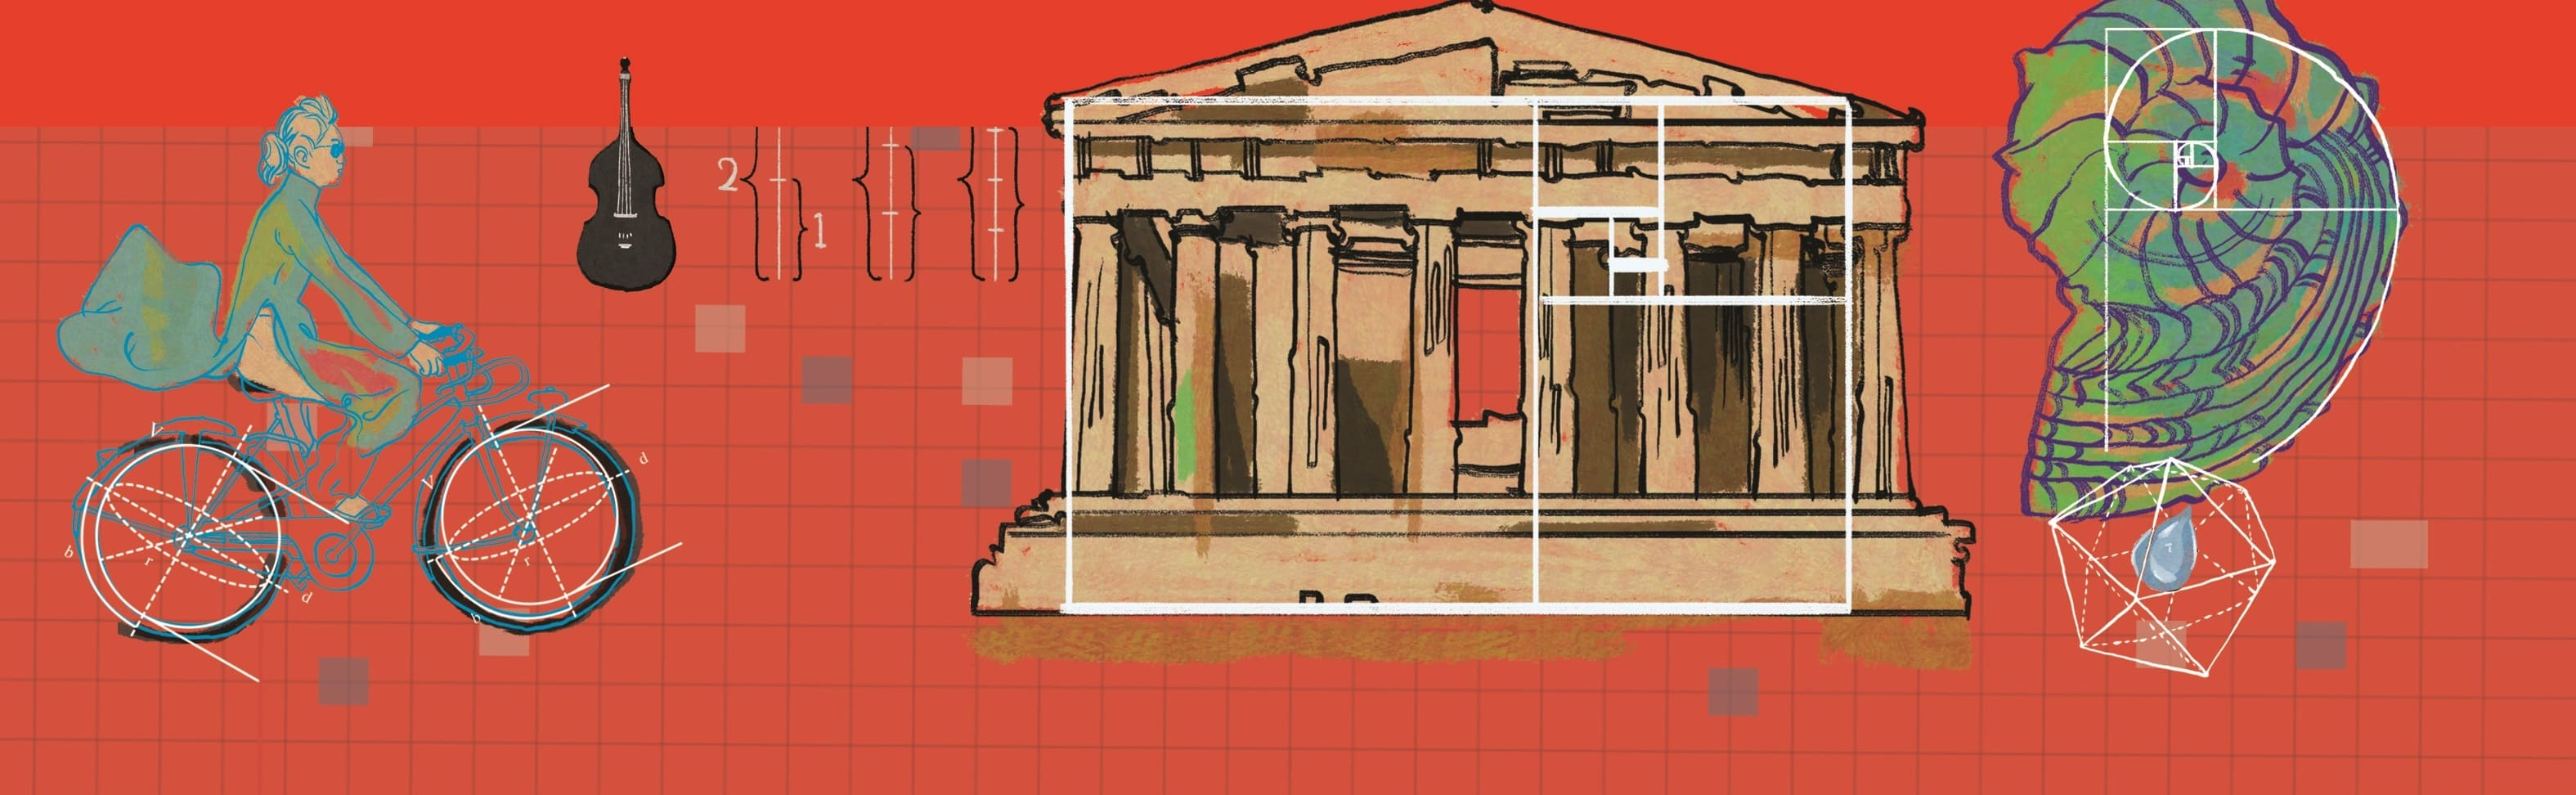
\includegraphics[width=19.3cm]{../bannertoanhocdoisong}}}
\AddToShipoutPicture*{\put(55,523){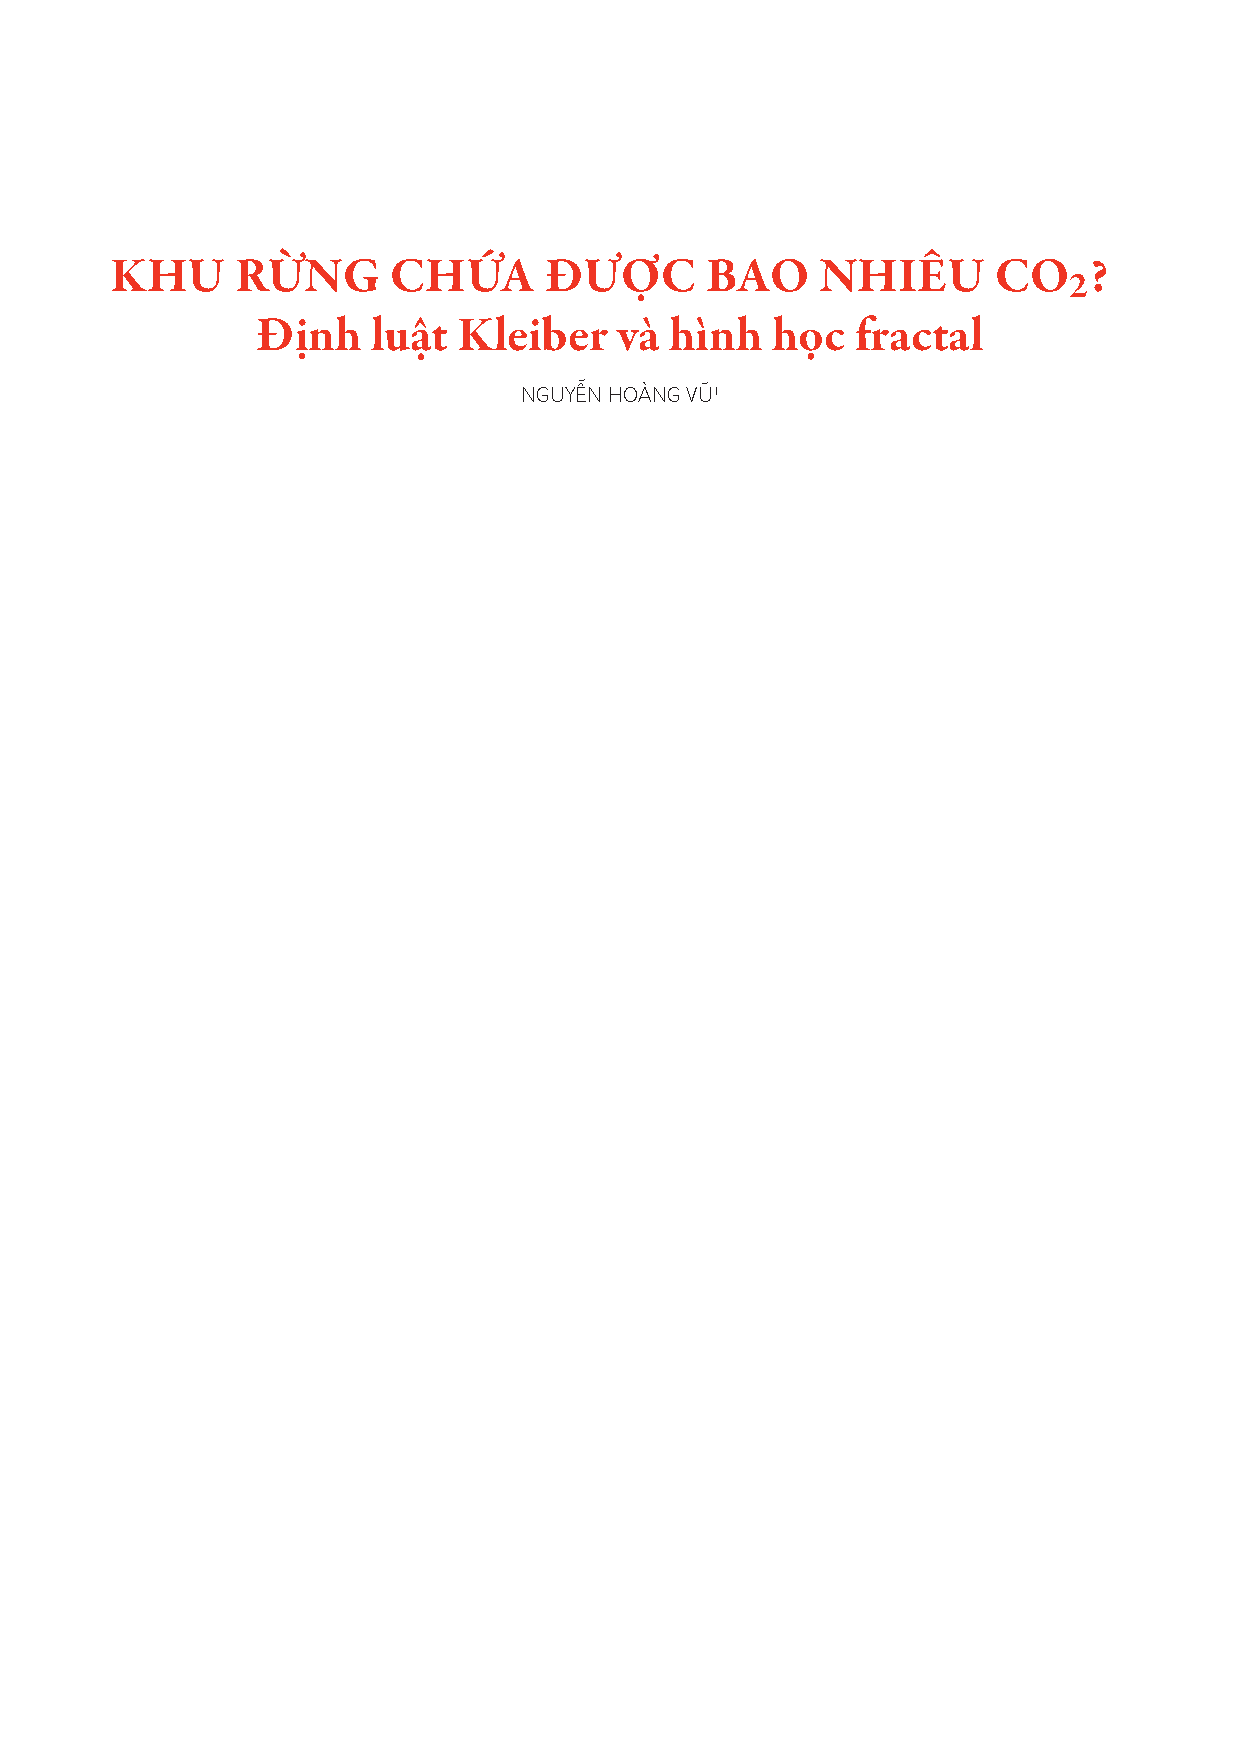
\includegraphics[scale=1]{../tieude2.pdf}}}
\centering
\endgroup

\vspace*{188pt}
\begin{multicols}{2}
	Cuộc cách mạng công nghiệp lần thứ tư (sau đây gọi tắt là CMCN $4{.}0$) với xu hướng phát triển dựa trên nền tảng tích hợp cao độ của hệ thống kết nối Số hóa -- Vật lý -- Sinh học và sự đột phá của Internet vạn vật, Trí tuệ nhân tạo đang tác động đến toàn thế giới. Cuộc cách mạng này được dự báo sẽ xóa nhòa khoảng cách giữa thế giới thực với thế giới ảo. Đặc biệt, mức độ ảnh hưởng, lan tỏa của cuộc cách mạng này sẽ nhanh hơn những gì đã xảy ra từ trước đến nay và làm thay đổi toàn bộ hệ thống sản xuất, quản lý, quản trị trên toàn thế giới. Cuộc cách mạng công nghiệp lần thứ nhất bắt đầu vào khoảng nửa sau thế kỷ thứ $18$ với nền tảng là máy móc cơ khí vận hành bằng động cơ hơi nước.
	\begin{figure}[H]
		\vspace*{-5pt}
		\centering
		\captionsetup{labelformat= empty, justification=centering}
		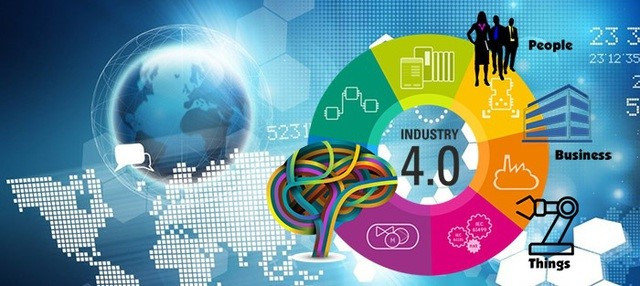
\includegraphics[width= 1\linewidth]{1a}
		\vspace*{-15pt}
	\end{figure}
	Cuộc cách mạng công nghiệp lần thứ hai vào khoảng nửa cuối thế kỷ thứ $19$ với nền tảng là động cơ đốt trong, động cơ điện và sản xuất theo dây chuyền. Cuộc cách mạng công nghiệp lần thứ ba được bắt đầu vào những năm $1960$ với nền tảng là công nghệ bán dẫn, điện tử, máy tính, tự động hóa. Cuộc cách mạng công nghiệp lần thứ tư được kế thừa từ Cuộc  cách mạng công nghiệp lần thứ ba và được đề cập nhiều từ những năm $2013$ với ba trụ cột chính là Kỹ thuật số, Sinh học và Vật lý.
	\vskip 0.05cm
	\textbf{\color{toanhocdoisong}Những đặc điểm nổi bật của CMCN $\pmb{4{.}0}$}
	\vskip 0.05cm
	Công nghệ trong kỷ nguyên CMCN $4{.}0$ có mức độ tự động hóa rất cao (so với mức độ tự động hóa của CMCN $3.0$), mô phỏng trí tuệ của con người. Trí tuệ nhân tạo (Artificial intelligence--AI) có thể tương tác với con người, thực hiện các hành vi thông minh như con người. Dựa trên các mô hình toán học và thuật toán phân tích dữ liệu lớn, AI có thể thay thế con người phân tích, tối ưu hóa, đưa ra quyết định và giải quyết vấn đề thay thế con người trong nhiều lĩnh vực, kể cả những lĩnh vực trước đây là độc quyền của con người như sáng tạo nghệ thuật v.v. 
	\vskip 0.05cm
	Công nghệ sinh học, công nghệ vật liệu trong CMCN $4.0$ có những bước tiến mang tính nhảy vọt, đột phá là nền tảng để tạo nên những tiến bộ vượt bậc trong lĩnh vực nông nghiệp, y học, dược liệu, năng lượng tái tạo… Vật lý hướng phát triển mạnh về nghiên cứu, chế tạo trang thiết bị công nghệ.
	\vskip 0.05cm
	Chuyển hóa thông tin từ thế giới thực (bao gồm cả các thực thể vật lý, xã hội và sinh học) sang thế giới ảo với dung lượng thông tin rất lớn, tốc độ cao và đa dạng về mọi mặt của đời sống tự nhiên và xã hội gắn với thuật ngữ chuyên môn là ``Dữ liệu lớn -- Big data". 
	\vskip 0.05cm
	Thông tin trong thế giới vật lý ảo này được kết nối với nhau và được quản lý, khai thác sử dụng bằng những hệ thống công nghệ số liên kết để xóa nhòa ranh giới không gian địa lý trên phạm vi toàn cầu và với tốc độ thời gian thực. Chúng ta luôn có được cái nhìn từ tổng quát toàn diện đến chi tiết thế giới hiện tại. Đây có thể coi là lời giải thích cho cụm từ chuyển đổi số hay nói cách khác chuyển đổi số là một xu hướng tất yếu của CMCN $4{.}0$.
	\vskip 0.05cm
	\textbf{\color{toanhocdoisong}Thế nào là chuyển đổi số (CĐS)}
	\vskip 0.05cm
	Khía cạnh công nghệ của CĐS là số hóa dữ liệu và ứng dụng dữ liệu dựa trên nền tảng kỹ thuật số. Công nghệ ở đây được hiểu là một hệ thống, trong đó có trang thiết bị kỹ thuật số, có các hệ thống xử lý kỹ thuật số, có dữ liệu đầu vào ở dạng số, có yêu tố con người, có yếu tố phương thức tổ chức hoạt động,  liên kết, tác động qua lại lẫn nhau và cho kết quả đầu ra là những sản phẩm có hiệu suất lớn về giá trị.
	\vskip 0.05cm
	Tuy nhiên với CĐS ở nghĩa rộng thì công nghệ không phải là yêu tố chính, mà là yếu tố kích thích. CĐS trong CMCN $4{.}0$ là quá trình hoàn chỉnh áp dụng số hóa và ứng dụng số hóa ở một cấp độ cao hơn và có quy mô lớn, là quá trình thay đổi phương thức kiến tạo, quản lý, điều hành, sử dụng dữ liệu truyền thống sang một phương thức kiến tạo, quản lý, điều hành, sử dụng dữ liệu dựa trên những nền tảng kỹ thuật số mới như: Dữ liệu lớn, Internet vạn vật, Trí tuệ nhân tạo, Điện toán đám mây, dựa vào lực lượng sản xuất mới, tiến bộ như đề cập ở trên trong mọi mặt trong đời sống xã hội với mục tiêu tạo nên một bước chuyển lớn về năng suất lao động và tổng giá trị sản xuất cho xã hội theo hướng bền vững và tích cực. Tóm lại CĐS trong CMCN $4{.}0$ là từ lực lượng sản xuất tiến bộ hiện đại, hình thành quan hệ sản xuất mới, phù hợp với mục tiêu xây dựng xã hội thịnh vương, hạnh phúc và tiến bộ. 
	\vskip 0.05cm
	\textbf{\color{toanhocdoisong}Chuyển đổi số ở nước ta}
	\vskip 0.05cm
	Tại Việt Nam, Đảng và Nhà nước ta đã sớm nhìn thấy cơ hội của CMCN $4{.}0$ và đã ban hành nhiều văn bản quan trong về chủ động tham gia vào CMCN $4{.}0$ (tiêu biểu là Nghị quyết $52$ của Bộ Chính Trị năm $2019$ về một số chủ trương, chính sách chủ động tham gia cuộc Cách mạng công  nghiệp lần thứ tư; Quyết định $749$ của Thủ tướng Chính phủ phê duyệt Chương trình Chuyển đổi số quốc gia đến năm $2025$ định hướng đến năm $2030$). Chương trình chuyển đổi số quôc gia theo Quyết định $749$ nhằm xây dựng ba trụ cột chính là Chính phủ số, Xã hội số và Kinh tế số.
	\vskip 0.05cm
	Hiện nay, cả trong công tác xây dựng/thực hiện chính sách lẫn trong hoạt động thực tiễn khái niệm CĐS đã trở nên phổ biến, lan tỏa trên toàn xã hội. Trong đó, doanh nghiệp và cơ quan quản lý nhà nước là những tổ chức tiên phong và xem CĐS là xu thế bắt buộc, tất yếu để nâng cao hiệu quả sản xuất kinh doanh, sức cạnh tranh và thực hiện thành công chiến lược xây dựng chính quyền số gắn với cải cách hành chính, xây dựng nền kinh tế số và xã hội thông minh trong thời kỳ cách mạng công nghiệp $4{.}0$.
	\vskip 0.05cm
	CĐS đối với doanh nghiệp và các cơ quan quản lý nhà nước giúp xây dựng nên những dữ liệu/tài nguyên số tạo thuận lợi cho việc quản lý, khai thác sử dụng. Dữ liệu số hóa đã trở thành tài sản của các doanh nghiệp và các cơ quan quản lý nhà nước. Dữ liệu ngày càng được bổ sung, liên kết, tích hợp với nhau giúp cải thiện, tăng cường hiệu năng quản lý nhà nước, quản trị xã hội theo hướng công khai, minh bạch, hiệu quả, tạo ra những thay đổi lớn trong chuỗi giá trị hàng hóa và cung ứng sản phẩm; tự động hóa, nâng cao hiệu suất công việc, hiệu quả sản xuất kinh doanh, năng lực cạnh tranh, gia tăng mạnh mẽ giá trị sản xuất, chất lượng dịch vụ công.
	\vskip 0.05cm
	Ví dụ việc tạo lập dữ liệu về dân cư, dữ liệu về tư pháp, dữ liệu về doanh nghiệp, người nộp thuế ... và kết nối liên thông những dữ liệu này sẽ giúp người dân, doanh nghiệp thực hiện những dịch vụ công được nhanh chóng, thuận tiện, không phải xuất trình nhiều loại giấy tờ liên quan khi có nhu cầu sử dụng dịch vụ hành chính công, trong khi vẫn bảo đảm được quyền riêng tư về cá nhân. Các dịch vụ công trực tuyến về y tế, giáo dục, tư pháp, hải quan, thuế, đăng ký kinh doanh ... sẽ cung cấp cho người dân, doanh nghiệp những tiện ích nhanh chóng, hạn chế tiếp xúc trực tiếp (tránh tiêu cực và giảm thiểu chi phí đi lại) với cơ quan hành chính trong công việc, cuộc sống và hoạt động sản xuất, kinh doanh của mình, trong khi vẫn tuân thủ các thủ tục hành chính theo qui định của pháp luật. Việc xây dựng chính phủ số trong đó lấy người dân là đối tượng phục vụ và dựa vào dữ liệu số sẽ góp phần tăng cường hiệu lực, hiệu quả quản lý nhà nước. Mặt khác, tiến trình này giúp đẩy mạnh sự phát triển công nghệ thông tin, công nghệ số trong nước, giúp phát triển cộng đồng doanh nghiệp công nghệ và nguồn nhân lực công nghệ có chất lượng ở nước ta.
	\vskip 0.05cm
	Các doanh nghiệp, khi áp dụng CĐS và tham gia vào nền kinh tế số sẽ xây dựng được các cách thức quản trị mới, hiệu quả hơn dựa vào tạo lập và khai thác nguồn thông tin số hóa. Họ cũng sẽ tiếp cận khách hàng và mở rộng thị trường nhanh hơn nhờ áp dụng thương mại điện tử và các chiến lược marketing tiên tiến dựa vào công nghệ phân tích dữ liệu lớn về xu hướng thị trường và nhu cầu ngày càng đa dạng của các tầng lớp khách hàng trong một xã hội số năng động và biến đông liên tục.
	\vskip 0.05cm
	Có thể khẳng định, CMCN $4{.}0$ và xu thế chuyển đổi số là tất yếu. Nó tạo ra vô vàn cơ hội cho mọi quốc gia, mọi đối tượng. Tuổi trẻ Việt Nam, đang được sống trong một đất nước năng động, hội nhập cần khẩn trương trang bị cho mình kiến thức và quyết tâm nắm bắt cơ hội, giành tấm vé lên chuyến tàu CMCN $4{.}0$ đang chuyển động cực kỳ nhanh này.
\end{multicols}
\vspace*{-10pt}
\rule{1\linewidth}{0.1pt}
\begingroup
\blfootnote{$^1$\color{toanhocdoisong}Hà Nội.}

\AddToShipoutPicture*{\put(100,268){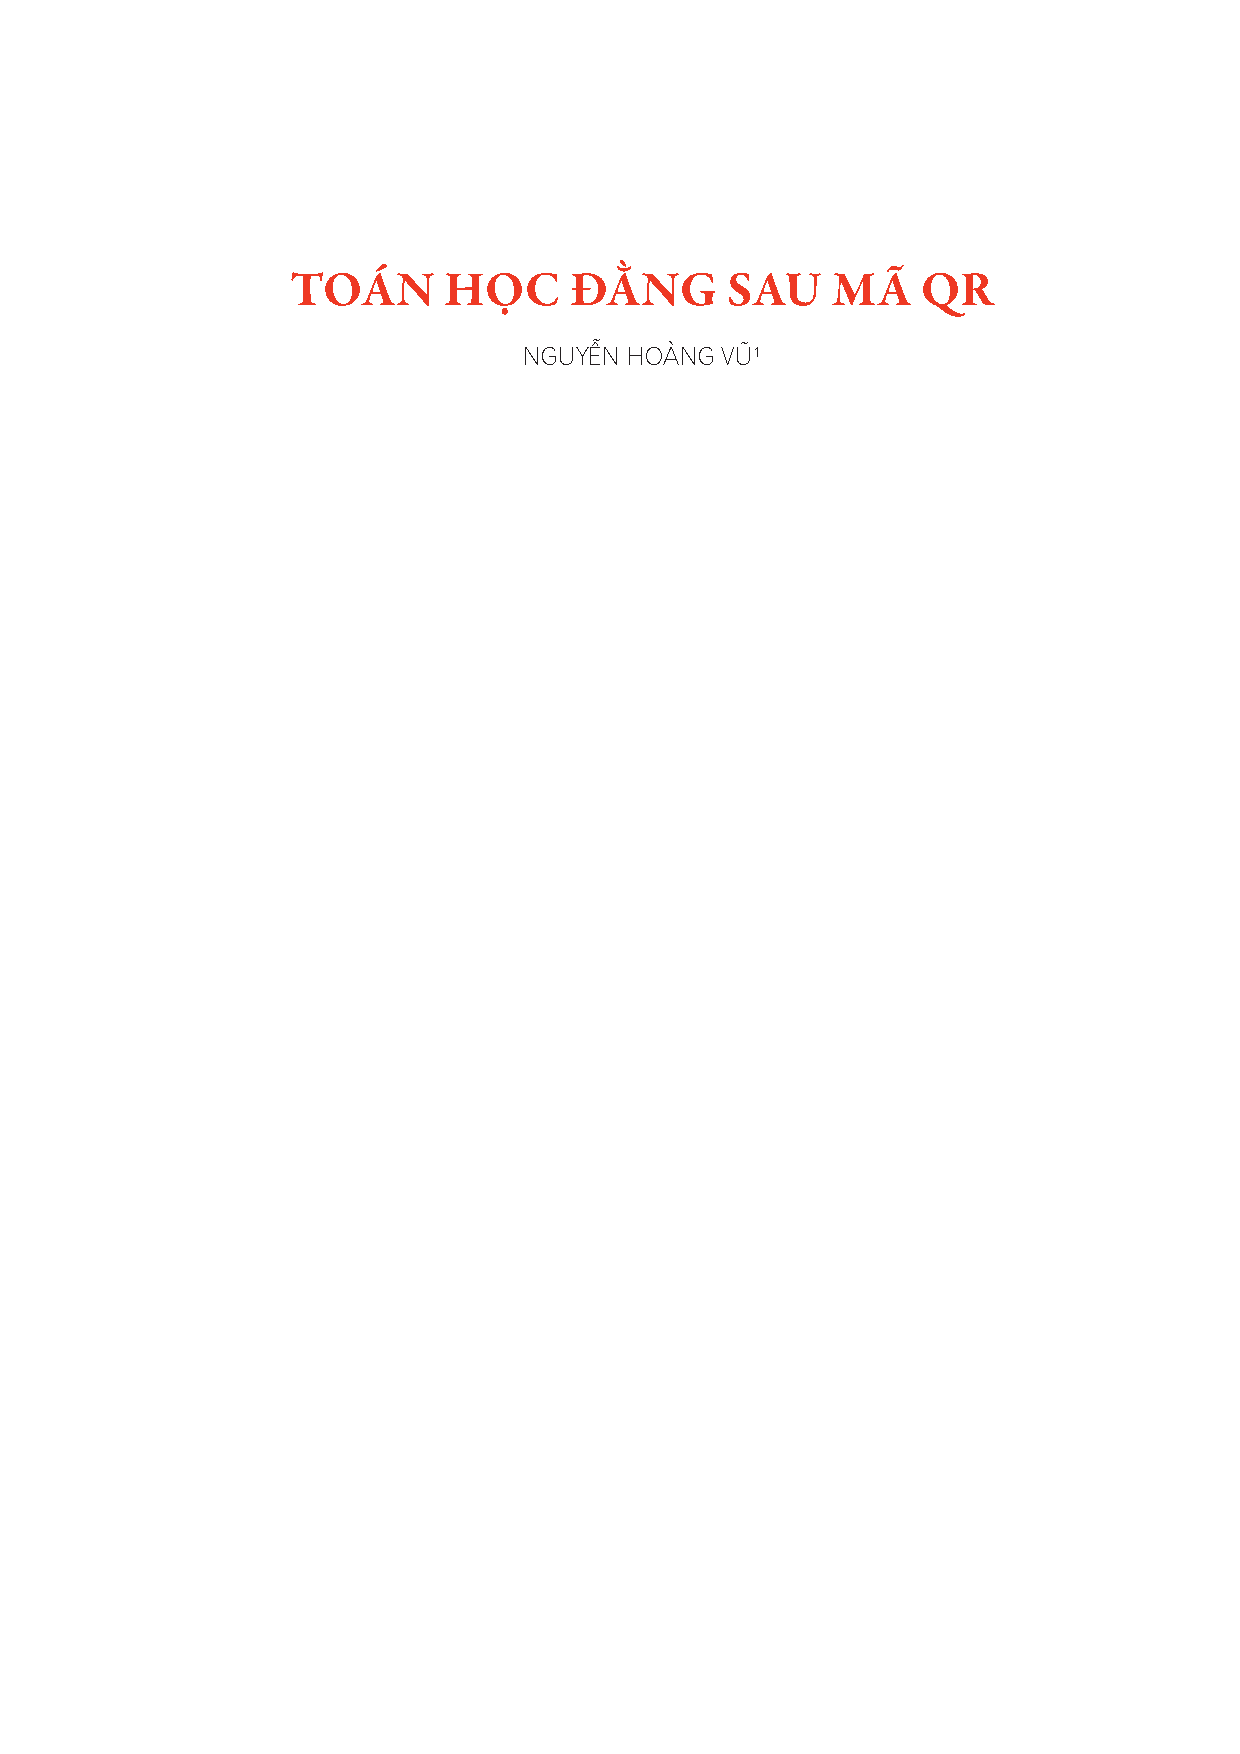
\includegraphics[scale=1]{../tieude3.pdf}}}
\centering
\endgroup

\vspace*{45pt}

\begin{multicols}{2}
	Mã QR đã trở nên rất quen thuộc trong đời sống hàng ngày quanh ta, mang lại sự tiện lợi lớn cho các hoạt động giao dịch cũng như trao đổi thông tin. Trong bài này, chúng ta hãy cùng tìm hiểu về vai trò của toán học trong quá trình xây dựng loại mã này.
	\vskip 0.05cm
	$\pmb{1.}$ \textbf{\color{toanhocdoisong}\color{toanhocdoisong}Mã sửa lỗi và sự ra đời của mã Reed -- Solomon}
	\vskip 0.05cm
	Một vấn đề không tránh khỏi khi thông tin được truyền tải từ nơi này đến nơi khác là việc nó có thể bị sai lệch trong quá trình truyền tin. Với các tín hiệu dạng nhị phân, một bit $0$ có thể biến thành $1$ và ngược lại. Xác suất của việc này phụ thuộc vào các đặc tính của đường truyền cũng như môi trường truyền dẫn.
	\vskip 0.05cm
	Để đảm bảo thông tin có thể được kiểm chứng đúng/sai, ta cần ghi thông tin theo một loại mã có thể giúp ta khẳng định nó có bị lỗi hay không. Loại mã này gọi là mã phát hiện lỗi.
	\vskip 0.05cm
	Một ví dụ về mã phát hiện lỗi là mã số của sách (ISBN) hoặc tạp chí (ISSN). Tạp chí Pi của chúng ta có mã ISSN là $2525-2437$. Trong $8$ chữ số của mã, chữ số cuối cùng được dùng để phát hiện lỗi. Đầu tiên, ta lấy $7$ chữ số đầu tiên, nhân mỗi một chữ số với số thứ tự tính từ bên phải (tức là $8$, $7$, $6$, $5$, ... $2$) rồi tính tổng:
	\setlength{\abovedisplayskip}{4pt}
	\setlength{\belowdisplayskip}{4pt}
	\begin{align*}
		&2\times8+5\times7+2\times6+5\times5+2\times4\\
		&+4\times3+3\times2=114.
	\end{align*}
	Lấy tổng này chia cho $11$ rồi lại lấy $11$ trừ đi số dư sẽ được chữ số cuối cùng (nếu giá trị này là $10$ thì ký tự cuối cùng là $X$): $114$ chia $11$ dư $4$; $11 - 4 = 7$.
	\vskip 0.05cm
	Nếu chữ số hoặc ký tự cuối không khớp với $7$ chữ số đầu tiên, ta có thể khẳng định rằng ISSN đã bị nhập sai. Cách làm này không chỉ phát hiện lỗi do một vị trí bị thay đổi mà còn phát hiện được trường hợp hai vị trí cạnh nhau bị hoán vị (một lỗi thường thấy khi con người nhập dữ liệu) thông qua hệ số khác nhau của các vị trí. Số $11$ được chọn do nó là một số nguyên tố, không chia hết cho bất cứ hệ số nào trong phép nhân. Nếu ta chọn số $10$, nó sẽ không phát hiện được lỗi nếu chữ số ở vị trí $5$ bị thay đổi một lượng chẵn.
	\vskip 0.05cm
	Trong nhiều trường hợp, chỉ phát hiện được lỗi là không đủ. Thay vì yêu cầu tín hiệu được gửi lại khi có lỗi, người ta muốn sử dụng một loại mã có thể giúp sửa lỗi khi lỗi được phát hiện. Muốn vậy, khi gửi tín hiệu, ta cần thêm một số thông tin khác để trợ giúp sửa lỗi.
	\vskip 0.05cm
	Một cách đơn giản nhất là gửi thông tin lặp. Thay vì gửi một bit có giá trị là $0$ hoặc $1$, ta có thể gửi nhiều bit có cùng giá trị. Chẳng hạn, nếu tín hiệu nhận được là $1101110111$, với quy định là $10$ bit liền nhau sẽ có cùng một giá trị, thì ta có thể khẳng định bit được gửi đi là $1$. Cách làm đơn giản này tuy có thể giúp sửa lỗi nhưng nó rất lãng phí đường truyền.
	\vskip 0.05cm
	Vậy cần phải truyền thêm bao nhiêu dữ liệu và dữ liệu sửa lỗi cần phải có dạng như thế nào? Đây là những vấn đề thiết yếu của ngành lý thuyết mã hóa.
	\vskip 0.05cm
	Năm $1948$, những nghiên cứu của nhà toán học Claude Shannon về entropy của thông tin cùng lượng thông tin cần truyền tối thiểu để sửa lỗi đã thúc đẩy nhiều nghiên cứu về các phương thức truyền thông tin có sửa lỗi.
	\vskip 0.05cm
	Một loại mã sửa lỗi quan trọng ra đời vào những năm $1950$ là mã Hamming (theo tên của nhà toán học R. W. Hamming). Ta hãy xét một trường hợp rất đơn giản với dữ liệu được truyền theo $3$ bit một, với $8$ tổ hợp: $000$, $001$, $010$, $011$, $100$, $101$, $110$, $111$. Nếu ta chọn cả $8$ tổ hợp này để truyền tin thì khi có một bit bị lỗi, ta không thể tiến hành phát hiện lỗi. Một cách đơn giản là chọn các trạng thái mà khi bị lỗi, ta có thể biết được giá trị gốc của tín hiệu.
	\begin{figure}[H]
		\vspace*{-10pt}
		\centering
		\captionsetup{labelformat= empty, justification=centering}
		\begin{tikzpicture}[toanhocdoisong,scale=0.7, node font=\small]
			\draw [] (-2.,1.)-- (1.4,0.);
			\draw [] (1.4,0.)-- (4.,1.);
			\draw [dashed] (4.,1.)-- (0.58,1.98);
			\draw [dashed] (0.58,1.98)-- (-2.,1.);
			\draw [] (-2.,1.)-- (-2.,4.5440090293338695);
			\draw [] (-2.,4.5440090293338695)-- (0.58,5.524009029333869);
			\draw [] (0.58,5.524009029333869)-- (4.,4.54400902933387);
			\draw [] (4.,4.54400902933387)-- (1.4,3.5440090293338695);
			\draw [] (1.4,3.5440090293338695)-- (-2.,4.5440090293338695);
			\draw [] (1.4,3.5440090293338695)-- (1.4,0.);
			\draw [] (4.,4.54400902933387)-- (4.,1.);
			\draw [dashed] (0.58,5.524009029333869)-- (0.58,1.98);
			\draw (-2.26,0.67) node {$(0,0,0)$};
			\draw (1.38,-0.35) node {$(1,0,0)$};
			\draw (4.25,0.55) node {$(1,1,0)$};
			\draw (-0.5,2.27) node {$(0,1,0)$};
			\draw (-2.36,4.89) node {$(0,1,1)$};
			\draw (0.5,6.11) node {$(0,1,1)$};
			\draw (2.25,3.35) node {$(1,0,1)$};
			\draw (4.32,4.91) node {$(1,1,1)$};
		\end{tikzpicture}
		\caption{\small\textit{\color{toanhocdoisong}Hình $1$. Các tổ hợp $3$ bit nhị phân biểu diễn theo dạng hình lập phương. Các đỉnh kề nhau sẽ khác biệt một bit.}}
		\vspace*{-10pt}
	\end{figure}
	Ta hãy biểu diễn $8$ tổ hợp trên $8$ đỉnh của hình lập phương. Có thể thấy khi đi từ một đỉnh đến một đỉnh kề nó thì có đúng một bit bị thay đổi. Số cạnh trên đường đi từ một đỉnh đến một đỉnh khác cho ta biết số bit bị thay đổi giữa hai trạng thái. Đây được gọi là khoảng cách Hamming giữa chúng. Ví dụ khoảng cách Hamming giữa $000$ và $101$ là $2$ còn khoảng cách giữa $000$ và $111$ là $3$.
	\vskip 0.05cm
	Giả sử trong môi trường truyền tin, tín hiệu $3$ bit bị lỗi tối đa một bit. Để có thể xác định được trạng thái gốc từ trạng thái lỗi, ta chỉ có thể chọn các đỉnh có khoảng cách là $3$. Do đó, chỉ có thể chọn $2$ đỉnh là $000$ và $111$. Giả sử tín hiệu nhận được là $011$, ta sẽ biết được tín hiệu gốc là $111$ do khoảng cách Hamming giữa chúng là $1$ còn khoảng cách Hamming giữa $011$ và $000$ là $2$. Khi đó, $000$ và $111$ được gọi là các codeword (từ mã) cho việc truyền tín hiệu. Trong trường hợp này ta truyền đi tổng cộng $3$ bit nhưng lượng thông tin chỉ có $2$ trạng thái (ứng với $2^1$ codeword) cho nên tốc độ truyền của ta là $1/3$. Nếu chọn tập hợp các đỉnh có khoảng cách giữa chúng là $2$ (ví dụ $4$ đỉnh $000$, $011$, $101$, $110$) để làm codeword thì ta chỉ có thể phát hiện lỗi chứ không sửa lỗi (ví dụ $001$ có khoảng cách đến $000$ và $011$ đều là $1$).
	\begin{table}[H]
		\vspace*{-5pt}
		\centering
		\captionsetup{labelformat= empty, justification=centering}
		\begin{tabular}{c c c c c c c c}
			\hline
			$1$ &$0$&$0$&$0$&$0$&$0$&$0$&$0$\\
			$2$ &$1$&$1$&$1$&$0$&$0$&$0$&$0$\\
			$3$ &$1$&$0$&$0$&$1$&$1$&$0$&$0$\\
			$4$ &$0$&$1$&$1$&$1$&$1$&$0$&$0$\\
			$5$ &$0$&$1$&$0$&$1$&$0$&$1$&$0$\\
			$6$ &$1$&$0$&$1$&$1$&$0$&$1$&$0$\\
			$7$ &$1$&$1$&$0$&$0$&$1$&$1$&$0$\\
			$8$ &$0$&$0$&$1$&$0$&$1$&$1$&$0$\\
			$9$ &$1$&$1$&$0$&$1$&$0$&$0$&$1$\\
			$10$ &$0$&$0$&$1$&$1$&$0$&$0$&$1$\\
			$11$ &$0$&$1$&$0$&$0$&$1$&$0$&$1$\\
			$12$ &$1$&$0$&$1$&$0$&$1$&$0$&$1$\\
			$13$ &$1$&$0$&$0$&$0$&$0$&$1$&$1$\\
			$14$ &$0$&$1$&$1$&$0$&$0$&$1$&$1$\\
			$15$ &$0$&$0$&$0$&$1$&$1$&$1$&$1$\\
			$16$ &$1$&$1$&$1$&$1$&$1$&$1$&$1$\\
			\hline
		\end{tabular}	
		\caption{\small\textit{\color{toanhocdoisong}Bảng $1$. $16$ codeword độ dài $7$ bit.}}
		\vspace*{-10pt}
	\end{table}
	Với mã Hamming, các quy tắc tính chẵn lẻ được tận dụng để thêm vào các thông tin cho phép sửa lỗi. Ta hãy xét một mã Hamming đơn giản với $7$ bit $b_1,b_2,\ldots,b_7$ theo quy tắc sau:
	\vskip 0.05cm
	$\bullet$ $b_1+b_3+b_5+b_7$ là chẵn
	\vskip 0.05cm
	$\bullet$ $b_2+b_3+b_6+b_7$ là chẵn
	\vskip 0.05cm
	$\bullet$ $b_4+b_5+b_6+b_7$ là chẵn
	\vskip 0.05cm
	Có tổng cộng $16$ codeword độ dài $7$ bit thỏa mãn các quy tắc trên (Bảng $1$). Đồng thời, các codeword này đều có khoảng cách Hamming giữa chúng là $3$.
	
	Khi giải mã tín hiệu, các tín hiệu vi phạm những quy tắc chẵn lẻ sẽ bị coi là lỗi. Việc phát hiện lỗi nằm ở bit nào (giả sử chỉ có $1$ bit bị lỗi) thì phức tạp hơn một chút. Tuy ta có thể dò xem codeword nào có khoảng cách ngắn nhất đến tín hiệu bị lỗi, việc này khá mất thời gian. Thay vì đó, người ta sử dụng dạng ma trận của các quy tắc được sử dụng để xây dựng mã (Bảng $2$).
	\begin{table}[H]
		\vspace*{-5pt}
		\centering
		\captionsetup{labelformat= empty, justification=centering}
		\begin{tabular}{ccccccc}
			\hline
			$b_1$ & $b_2$& $b_3$& $b_4$&$b_5$ &$b_6$ &$b_7$\\
			\hline
			$1$ & $0$&$1$&$0$&$1$&$0$&$1$\\
			$0$ & $1$&$1$&$0$&$0$&$1$&$1$\\
			$0$ & $0$&$0$&$1$&$1$&$1$&$1$\\
		\end{tabular}	
		\caption{\small\textit{\color{toanhocdoisong}Bảng $2$. Ma trận ứng với $3$ quy tắc trong mã Hamming mà ta đang xét.}}
		\vspace*{-10pt}
	\end{table}
	Ví dụ, với chuỗi tín hiệu lỗi $1101101$, nó vi phạm quy tắc $1$ và $3$. Ta cần tìm cột trong ma trận mà khi bit ứng với cột này bị lật ngược lại thì chỉ có quy tắc $1$ và $3$ bị ảnh hưởng còn quy tắc $2$ không thay đổi. Nói cách khác, ta cần tìm cột có dạng:
	\begin{align*}
		1\\[-0.5ex]
		0\\[-0.5ex]
		1
	\end{align*}
	tức là cột thứ $5$ trong ma trận. Do đó, có thể kết luận bit thứ $5$ bị lỗi và codeword gốc là $1101001$.
		\begin{figure}[H]
		\vspace*{-5pt}
		\centering
		\captionsetup{labelformat= empty, justification=centering}
		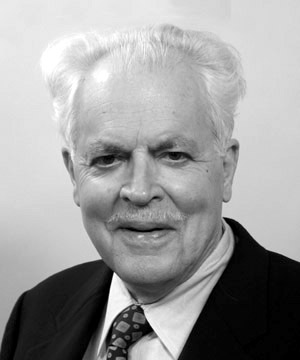
\includegraphics[height= 0.575\linewidth]{2}
		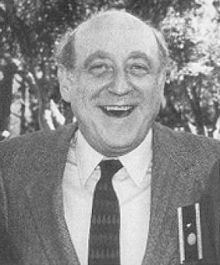
\includegraphics[height= 0.575\linewidth]{3}
		\caption{\small\textit{\color{toanhocdoisong}Trái: Irving Reed ($1923 - 2012$). Phải: Gustave Solomon ($1930 - 1996$).}}
		\vspace*{-10pt}
	\end{figure}
	Mã Hamming $7$ bit trên có $2^4=16$ codeword, tức là khi truyền đi $7$ bit, ta thu được lượng thông tin tương đương với $4$ bit. Tốc độ truyền ở đây là $4/7$. Tùy theo nhu cầu, người ta có thể thiết kế các mã Hamming với khoảng cách giữa các codeword lớn hơn để có thể sửa lỗi cho nhiều hơn $1$ bit.
	\vskip 0.05cm
	Sau khi Hamming đưa ra mã sửa lỗi thực tiễn đầu tiên sử dụng các kỹ thuật đại số tuyến tính như trên, cuộc đua giữa các nhà toán học để tìm ra những cách mã hóa tốt hơn trở nên sôi động. Một dấu ấn quan trọng của ngành mã hóa là sự ra đời của mã Reed -- Solomon, được hai nhà toán học Irving Reed và Gustave Solomon công bố năm $1960$. Mã này sử dụng các cấu trúc đại số phức tạp hơn bao gồm trường Galois cùng các đa thức trên trường này (xem chi tiết ở phần phụ lục). Với nhiều lợi thế so với mã Hamming về khả năng sửa lỗi cũng như tốc độ truyền, mã Reed -- Solomon đã có nhiều ứng dụng rộng rãi trong các lĩnh vực của đời sống. Một trong số những ứng dụng đó chính là mã QR. 
	\vskip 0.05cm
	$\pmb{2.}$ \textbf{\color{toanhocdoisong}\color{toanhocdoisong}Mã QR}
%	\vskip 0.05cm
	\begin{figure}[H]
			\vspace*{-5pt}
			\centering
			\captionsetup{labelformat= empty, justification=centering}
			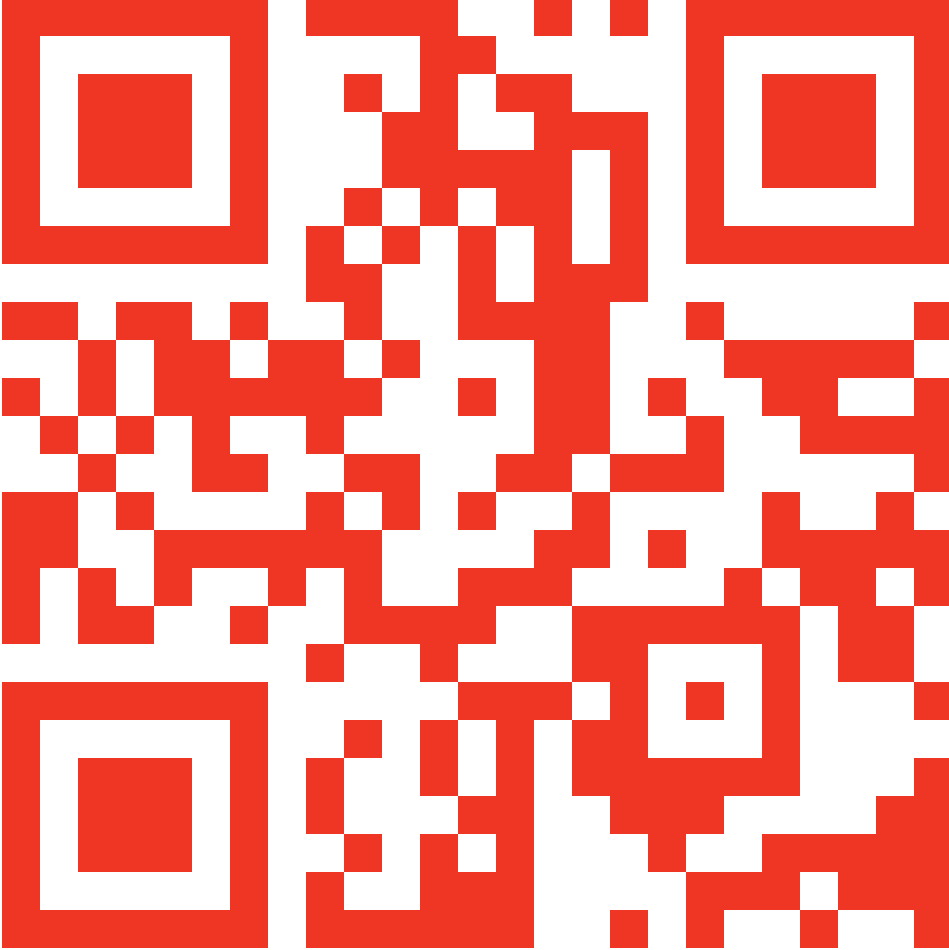
\includegraphics[width= 0.7\linewidth]{QR}
			\caption{\small\textit{\color{toanhocdoisong}Hình $2$. Mã QR của Tạp chí Pi.}}
			\vspace*{-10pt}
		\end{figure}
	Mã QR (viết tắt của Quick Response) mà chúng ta quen thuộc được kỹ sư người Nhật, Masahiro Hara thiết kế năm $1994$ khi làm tại công ty Denso Wave. Lúc đó, Masahiro được giao nhiệm vụ thiết kế một loại mã mới để thay thế mã dạng barcode (mã vạch) (Hình $3$). Tuy mã barcode đã được dùng rất phổ biến trong cả sản xuất lẫn phân phối, nhưng vì nó ghi lại thông tin theo một chiều nên dung lượng thông tin của barcode ($20$ ký tự) đã không còn đáp ứng được nhu cầu thực tế với sự đa dạng hóa sản xuất đầu những năm $1990$ ở Nhật. Để lưu trữ những thông tin dài, người ta thường phải sử dụng nhiều barcode cùng lúc và do đó phải tiến hành quét nhiều lần cho mỗi sản phẩm.
	\begin{figure}[H]
		\vspace*{-10pt}
		\centering
		\captionsetup{labelformat= empty, justification=centering}
		$a)$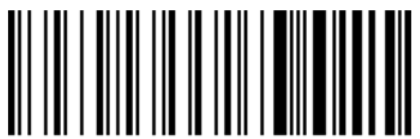
\includegraphics[width= 0.8\linewidth]{4}
		$b)$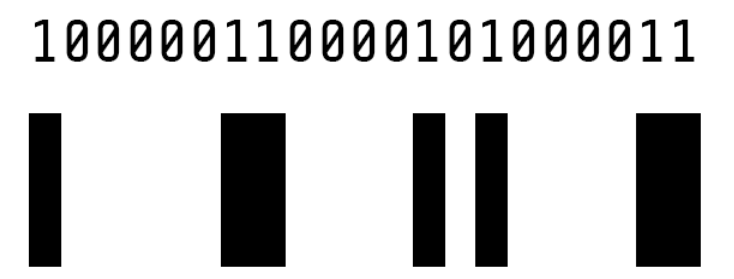
\includegraphics[width= 0.8\linewidth]{5}
		\caption{\small\textit{\color{toanhocdoisong}Hình $3.$ $a)$ Mã barcode gồm cách vạch với độ dày và khoảng cách khác nhau. $b)$ Thực chất của mã barcode là các cột màu trắng hoặc đen liên tiếp ứng với các bit $0$ hoặc $1$ để biểu diễn thông tin đã được chuyển từ dạng ký tự sang dạng bit.}}
		\vspace*{-10pt}
	\end{figure}
	Để có thể chứa được nhiều thông tin hơn, Masahiro quyết định sử dụng mã dạng hình vuông (hai chiều không gian thay vì một chiều như barcode). Vấn đề đầu tiên là làm thế nào để thiết bị có thể nhận diện được vùng mã khi quét. Masahiro đã nảy ra ý tưởng đưa thêm các hình hình học vào các góc để giúp định vị mã.
	\vskip 0.05cm
	Tuy nhiên, việc chọn hình hình học này thế nào cũng là vấn đề khó bởi trong thực tế có thể có các hình hình học khác ở gần mã của ta làm phần mềm không thể nhận diện được mã một cách chính xác. Sau một thời gian nghiên cứu về tỷ lệ giữa các vùng trắng/đen trong các nội dung  ảnh hoặc văn bản trên báo, tạp chí, tờ rơi, thùng carton, và nhiều tài liệu khác; nhóm làm việc của Masahiro quyết định sử dụng hình ô vuông như ta thấy ở ba góc của mã QR ngày nay. Hình ô vuông này có tỷ lệ các phần đen/trắng khi quét theo các góc khác nhau đều là $1 : 1 : 3 : 1 : 1$. Theo kết quả thống kê thì tỷ lệ này ít xuất hiện nhất trên các vật liệu in thực tế nên mã QR sẽ không bị lẫn vào môi trường xung quanh và có thể được thiết bị quét nhận diện tự động nhanh chóng sau khi tiến hành quét.
	\begin{figure}[H]
		\vspace*{-10pt}
		\centering
		\captionsetup{labelformat= empty, justification=centering}
		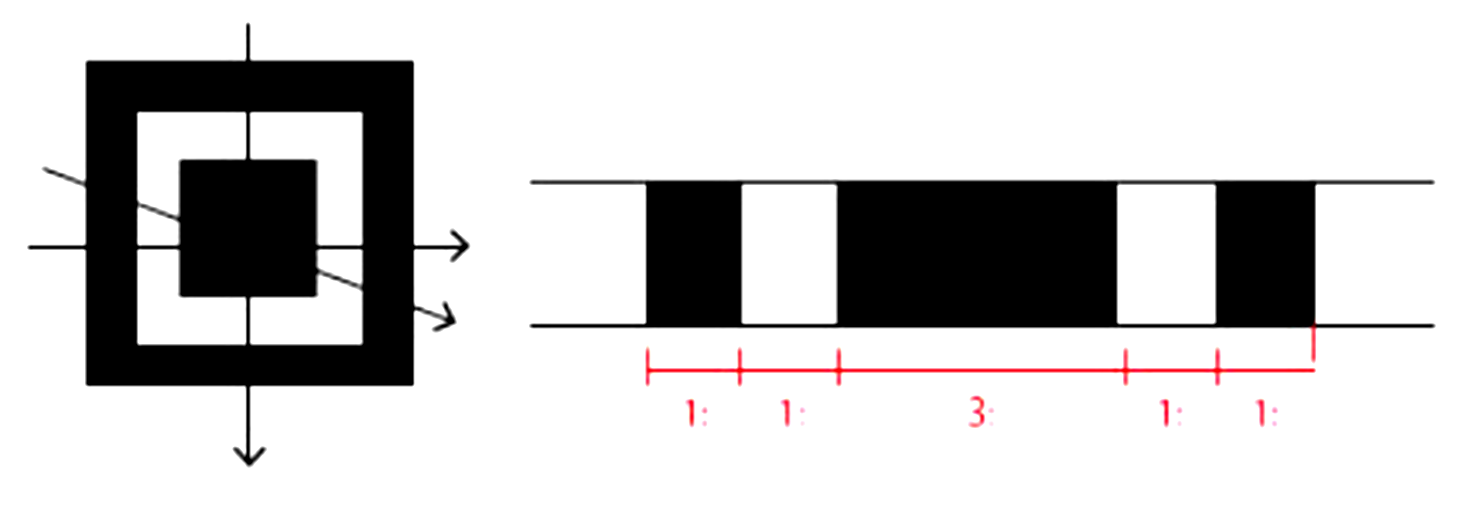
\includegraphics[width=1\linewidth]{6}
		\caption{\small\textit{\color{toanhocdoisong}Hình $4$. Ô vuông định vị cho mã QR và tỷ lệ đen/trắng khi quét.}}
		\vspace*{-10pt}
	\end{figure}
	Một vấn đề thực tế khác mà Masahiro muốn giải quyết với mã QR là tình trạng các vết bẩn làm sai lệch thông tin. Trong các môi trường như nhà xưởng, cửa hàng, ... mã đã in ra có thể dễ dàng bị dính các loại dầu, bụi đất, ... Để việc đọc mã có thể tiến hành thuận lợi trong các điều kiện này, ông sử dụng mã sửa lỗi Reed -- Solomon để ghi thông tin thay vì chuyển trực tiếp từ dạng ký tự sang dạng bit như mã barcode. Do đó, thông tin bị sai lệch ở mức độ cho phép trong quá trình quét có thể được sửa lại thay vì phải quét lại hoặc làm sạch vùng chứa mã.
	\begin{figure}[H]
		\vspace*{-5pt}
		\centering
		\captionsetup{labelformat= empty, justification=centering}
		$a)$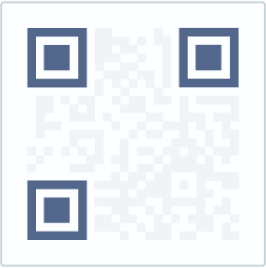
\includegraphics[height=0.35\linewidth]{7}
		$b)$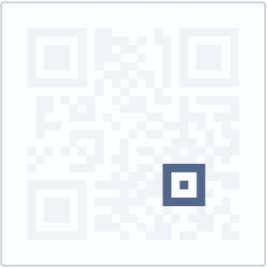
\includegraphics[height=0.35\linewidth]{8}
		$c)$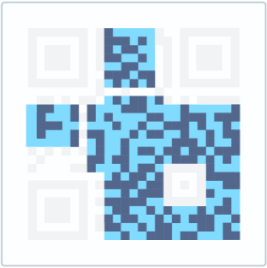
\includegraphics[height=0.35\linewidth]{9}
		$d)$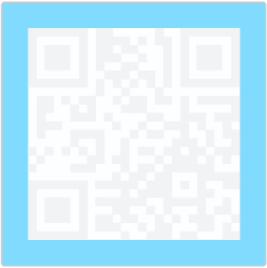
\includegraphics[height=0.35\linewidth]{10}
		\caption{\small\textit{\color{toanhocdoisong}Hình $5$. Một số thành phần của mã QR. $a)$ Các ô định vị. $b)$ Ô vuông gióng hàng. $c)$ Phần ghi dữ liệu. $d)$ Phần viền trắng.}}
		\vspace*{-10pt}
	\end{figure}
	Từ khi được Masahiro thiết kế đến nay, mã QR đã trải qua nhiều phiên bản. Về cơ bản, một mã QR gồm các nội dung như trong Hình $5$. Ngoài các ô vuông định vị và phần thông tin sử dụng mã Reed -- Solomon, mã QR còn gồm một số thành phần khác như ô vuông gióng hàng, phần viền trắng (để tách biệt với xunh quanh) và các phần ghi một số thông tin khác về phiên bản mã và định dạng mã, ...
	\begin{figure}[H]
		\vspace*{-5pt}
		\centering
		\captionsetup{labelformat= empty, justification=centering}
		
\includegraphics[height=0.35\linewidth]{11}
		
		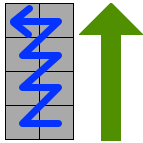
\includegraphics[height=0.33\linewidth]{12}
		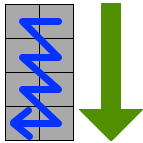
\includegraphics[height=0.33\linewidth]{13}
		\caption{\small\textit{\color{toanhocdoisong}Hình $6$. Thông tin sau khi được mã hóa theo mã Reed -- Solomon sẽ được ghi theo các làn như hình vẽ (trên). Ứng với mỗi chiều trong làn, thông tin sẽ được ghi trong hai cột (dưới) với màu đen đại diện bit $1$ còn màu trắng đại diện bit $0$.}}
		\vspace*{-10pt}
	\end{figure}
	Khi mã hóa, các thông tin thực tế (chữ số, ký tự, ...) đã được chuyển thành dạng bit nhị phân theo quy tắc định trước (tùy theo phiên bản mã QR) sẽ được mã hóa thành mã Reed -- Solomon dạng bit. Các bit được ghi lên trên hình vuông theo cách thức như trong Hình $6$. Vị trí đen ứng với bit $1$ còn vị trí trắng ứng với bit $0$.
	
	Khi thiết bị quét mã QR, phần mềm sẽ định vị mã dựa vào vị trí của các ô vuông đánh dấu và tiến hành quét phần dữ liệu. Dữ liệu sau khi quét được tiến hành giải mã theo thuật toán giải mã của mã Reed -- Solomon. Do khả năng sửa lỗi của mã này nên nếu quá trình quét có một số bit bị nhận diện sai (đen thành trắng hoặc trắng thành đen), phần mềm vẫn có thể tiến hành sửa lỗi để cho ra thông tin ban đầu. Nếu số lượng lỗi vượt quá khả năng sửa lỗi của thuật toán, người dùng phải tiến hành quét lại.
	\begin{figure}[H]
		\vspace*{-5pt}
		\centering
		\captionsetup{labelformat= empty, justification=centering}
		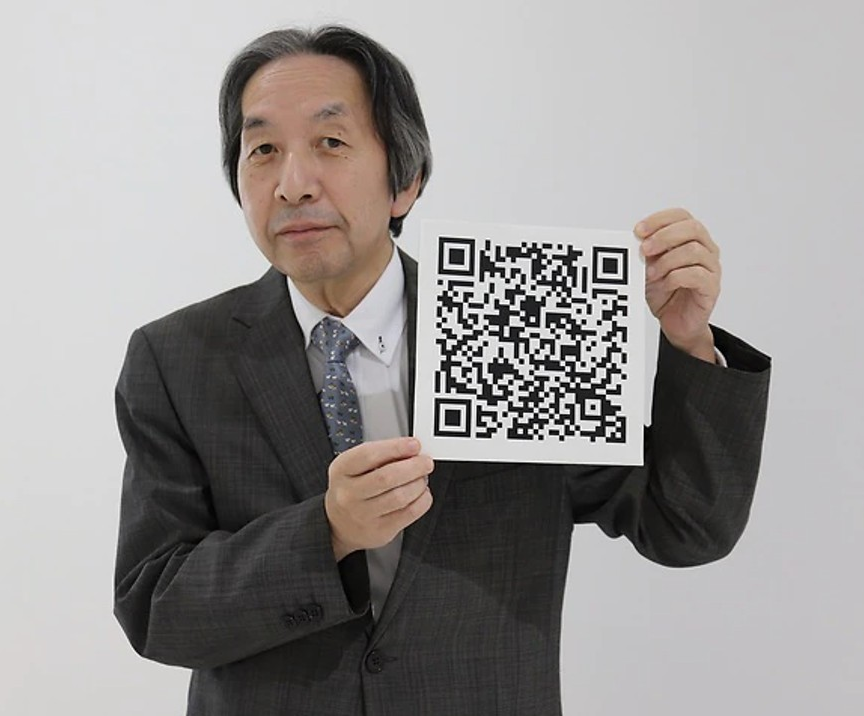
\includegraphics[width= 1\linewidth]{14}
		\caption{\small\textit{\color{toanhocdoisong}Hình $7a$. Masahiro và mã QR do ông phát minh.}}
		\vspace*{-5pt}
	\end{figure}
	\begin{figure}[H]
		\vspace*{5pt}
		\centering
		\captionsetup{labelformat= empty, justification=centering}
		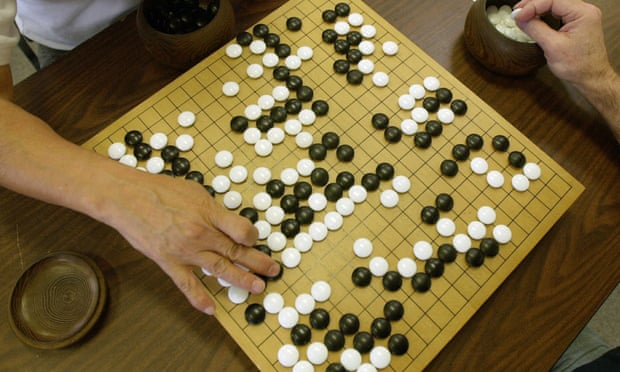
\includegraphics[width= 1\linewidth]{15}
		\caption{\small\textit{\color{toanhocdoisong}Hình $7b$. Masahiro có ý tưởng về các ô đen trắng cho mã QR từ trò chơi Go (cờ vây) mà ông hay chơi trong giờ nghỉ.}}
		\vspace*{-10pt}
	\end{figure}
	Ngày nay, với sự phổ biến của các thiết bị điện thoại thông minh, mã QR đã xuất hiện không chỉ ở trong các dây chuyền sản xuất mà còn được ứng dụng ở rất nhiều hoạt động của đời sống trên thế giới, từ thanh toán ngân hàng đến các giao dịch ở cửa hàng, siêu thị, bệnh viện, phương tiện công cộng, ... Nó cũng có vai trò quan trọng trong việc truy vết COVID $19$ ở nhiều nơi trên thế giới trong thời gian vừa qua; bản thân Masahiro cũng nói rằng ông cảm thấy rất hài lòng về sự đóng góp này của mã QR.
	\begin{figure}[H]
		\vspace*{-5pt}
		\centering
		\captionsetup{labelformat= empty, justification=centering}
		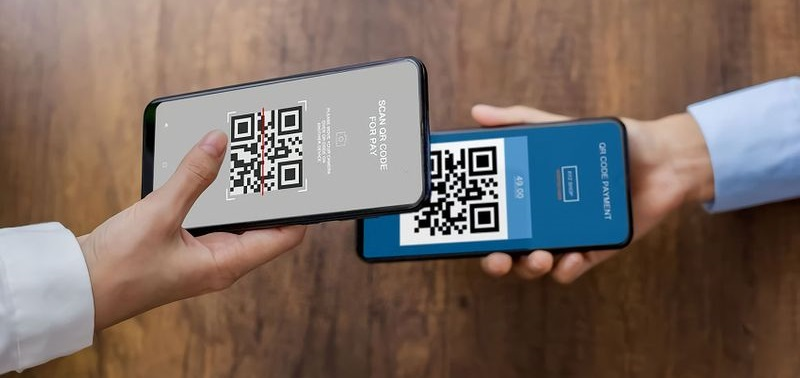
\includegraphics[width= 1\linewidth]{16}
		\caption{\small\textit{\color{toanhocdoisong}Hình $8$. Việc sử dụng mã QR giúp tiến hành các giao dịch không cần tiền mặt chỉ với điện thoại di động.}}
		\vspace*{-10pt}
	\end{figure}
	$\pmb{3.}$ \textbf{\color{toanhocdoisong}\color{toanhocdoisong}Một số ứng dụng khác của mã Reed -- Solomon}
	\vskip 0.05cm
	Mã Reed -- Solomon đã từ lâu được sử dụng để mã hóa dữ liệu cho các loại đĩa lưu trữ thường thấy trong đời sống như CD, DVD, MiniDisc và Blu--ray. Dữ liệu nhị phân sau khi chuyển thành mã Reed -- Solomon sẽ được ghi lên bề mặt đĩa tạo thành các rãnh lồi lõm. Khi đầu đọc đọc lại các bit này, chúng sẽ được giải mã theo thuật toán giải mã tương ứng để cho ra dữ liệu ban đầu. Do khả năng khôi phục lỗi của mã Reed -- Solomon, ngay cả khi có lỗi lúc đọc (thường do bề mặt đĩa bị bụi, bẩn, ...), hệ thống vẫn có thể khôi phục dữ liệu gốc.
	\begin{figure}[H]
		\vspace*{-5pt}
		\centering
		\captionsetup{labelformat= empty, justification=centering}
		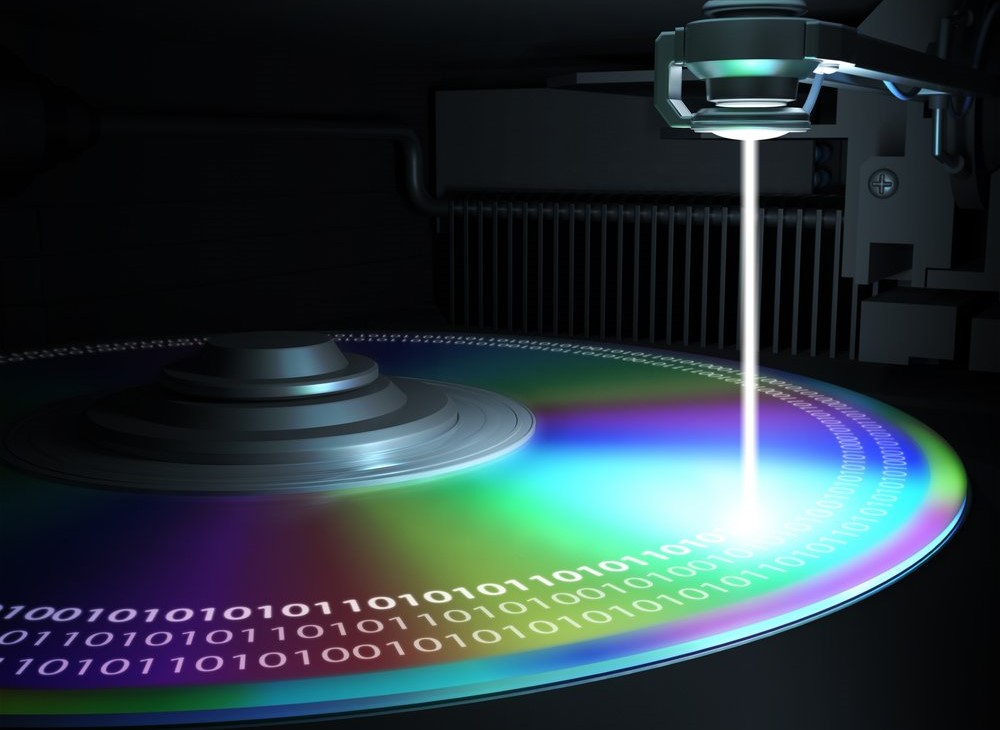
\includegraphics[width= 1\linewidth]{17}
		\caption{\small\textit{\color{toanhocdoisong}Hình $9$. Dữ liệu được mã hóa thành mã Reed - Solomon trước khi ghi trên bề mặt của các đĩa quang học.}}
		\vspace*{-10pt}
	\end{figure}
	Mã Reed -- Solomon cũng được sử dụng để mã hóa dữ liệu cho việc truyền tin của ngành viễn thông, theo dây cáp lẫn vô tuyến. Đặc biệt, mã này được sử dụng trên các thiết bị thăm dò không gian của NASA như tàu thăm dò Voyager $1$ và nhiều tàu thăm dò sau~đó.
	\begin{figure}[H]
		\vspace*{-5pt}
		\centering
		\captionsetup{labelformat= empty, justification=centering}
		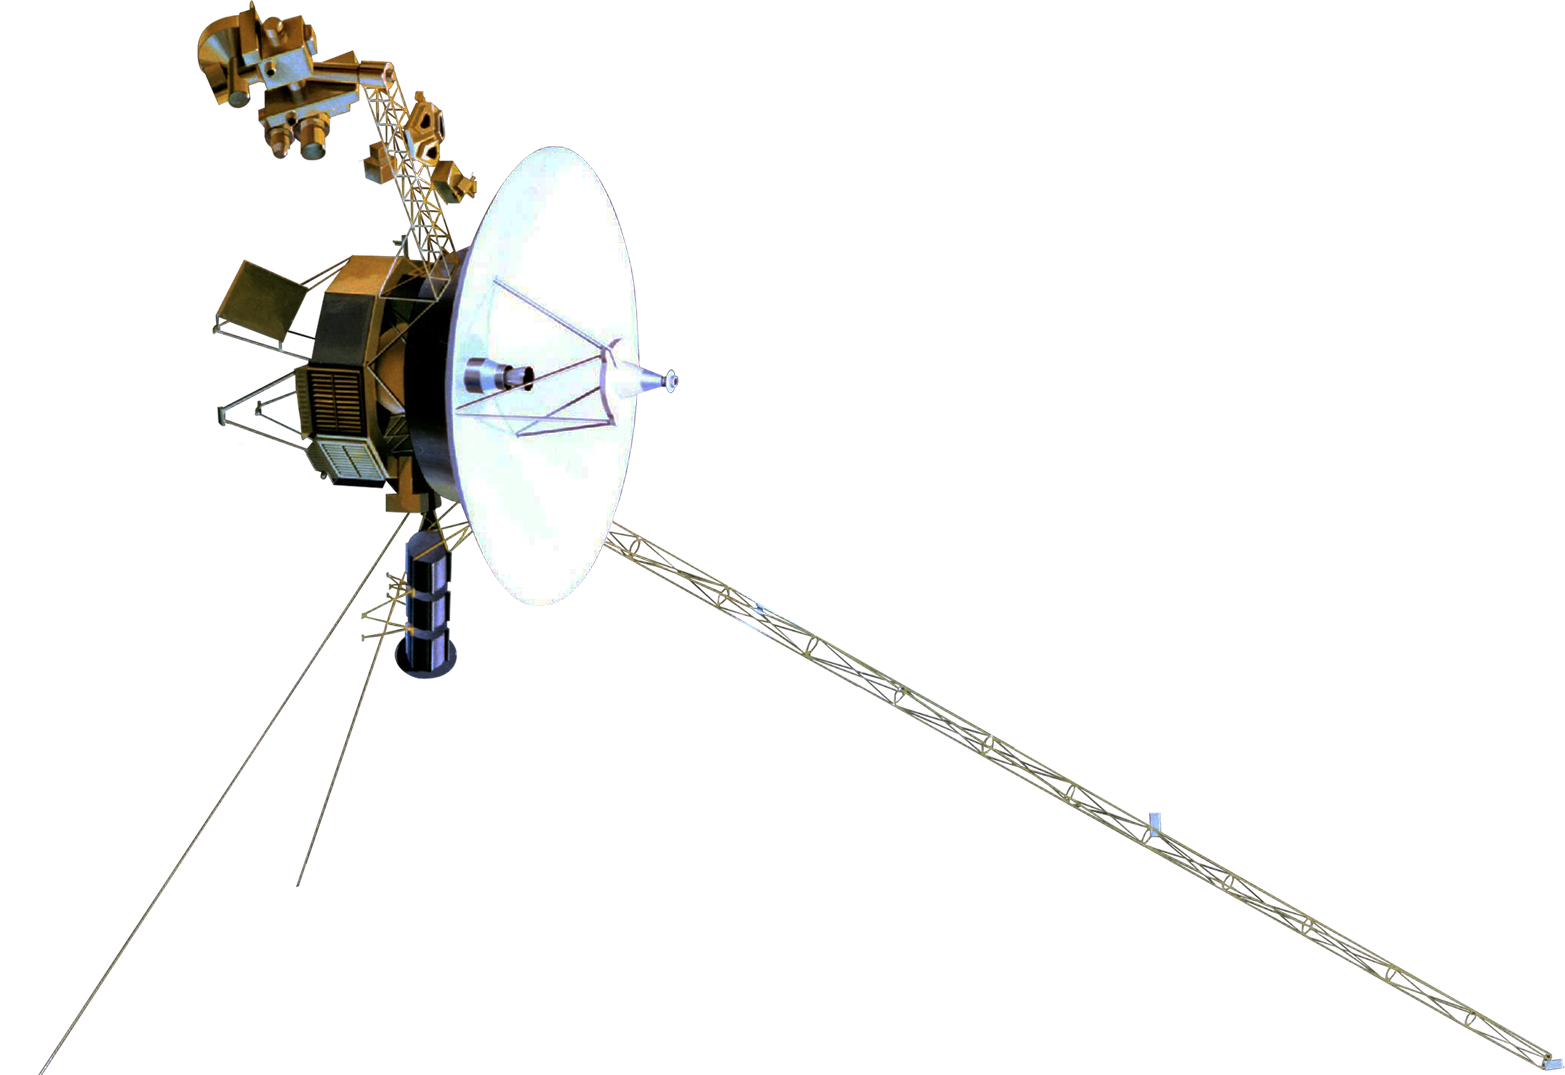
\includegraphics[width= 0.95\linewidth]{18}
		\caption{\small\textit{\color{toanhocdoisong}Hình $10$. Tàu thăm dò Voyager $1$ của NASA.}}
		\vspace*{-10pt}
	\end{figure}
	Mã Reed -- Solomon còn xuất hiện ở các hệ thống lưu trữ trong trung tâm dữ liệu. Trong kết nối ổ cứng theo dạng RAID $6$, các mã Reed -- Solomon để sửa lỗi cho dữ liệu của mỗi ổ cứng sẽ được hệ thống phân bố ở các ổ khác. Nếu một ổ cứng bị hỏng, dữ liệu có thể được khôi phục từ dữ liệu cùng các mã Reed -- Solomon ở trong các ổ cứng còn lại. 
	\begin{figure}[H]
		\vspace*{-5pt}
		\centering
		\captionsetup{labelformat= empty, justification=centering}
		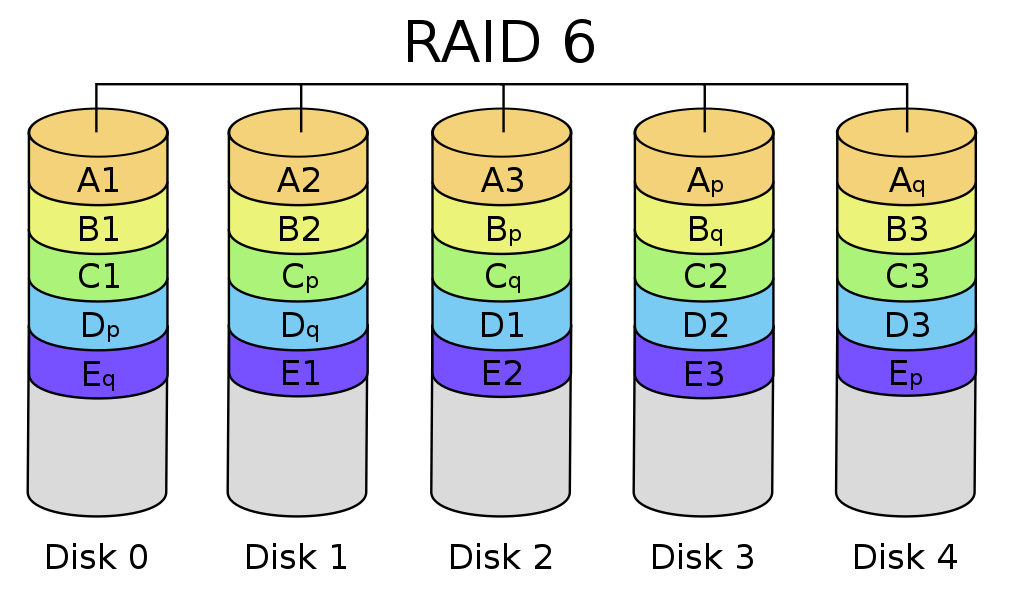
\includegraphics[width= 1\linewidth]{19}
		\caption{\small\textit{\color{toanhocdoisong}Hình $11$. Lưu trữ dữ liệu trên $5$ ổ cứng theo dạng RAID $6$. Dữ liệu cũng như thông tin sửa lỗi được chia ra để lưu trữ ở các ổ cứng khác nhau để cho phép phục hồi trong trường hợp một trong các ổ cứng này bị hỏng.}}
		\vspace*{-10pt}
	\end{figure}
	$\pmb{4.}$ \textbf{\color{toanhocdoisong}\color{toanhocdoisong}Lời kết}
	\vskip 0.05cm
	Sự xuất hiện của trường Galois dưới dạng cơ sở lý thuyết của mã Reed -- Solomon cho thấy ngay cả những khái niệm trừu tượng và phức tạp trong toán học cũng có thể đóng vai trò quan trọng trong ứng dụng thực tiễn nếu ta tiến hành mô hình hóa bài toán một cách phù hợp. Mã Reed -- Solomon cũng như các ứng dụng đa dạng của nó sẽ không xuất hiện nếu không có những nghiên cứu toán học thuần túy từ hơn một thế kỷ trước đó của Galois. Ngày nay, lĩnh vực lý thuyết mã hóa vẫn còn rất nhiều vấn đề toán học thú vị khác với nhiều cơ hội cho những ai muốn tìm tòi khám phá.
	\vskip 0.05cm
	\textbf{\color{toanhocdoisong}Phụ lục. Trường Galois và mã Reed -- Solomon}
	\vskip 0.05cm
	Trong đại số, trường là một tập hợp mà trên đó có thể định nghĩa phép cộng và phép nhân với các tính chất giao hoán và kết hợp. Đồng thời, trong trường phải tồn tại phần tử $0$ và $1$ sao cho với phần tử $a$ bất kỳ của trường thì $a+0=a$; $a\cdot1=1$. Mỗi phần tử của trường đều phải có phần tử đối (với phép cộng) và phần tử nghịch đảo (với phép nhân, trừ trường hợp nghịch đảo của $0$) cũng nằm trong trường này.
	\vskip 0.05cm
	Ví dụ, tập hợp các số nguyên $\mathbb{Z}$ không phải là một trường vì nghịch đảo của một số nguyên có thể không phải là một số nguyên. Trong khi đó, tập hợp các số hữu tỷ $\mathbb{Q}$ hay tập hợp các số thực $\mathbb{R}$ đều là một trường.
	\vskip 0.05cm
	Trường Galois (còn gọi là trường hữu hạn), được đặt tên theo nhà toán học Evariste Galois, là một trường có số phần tử là hữu hạn. Trường Galois $GF(q)$ (có $q$ phần tử) luôn chứa một phần tử $\alpha$ sao cho cả các phần tử khác $0$ của trường đều là các lũy thừa của $\alpha$: $\{1,\alpha,\alpha^2,\ldots,\alpha^{q-2}\}$. Khi đó ta cũng có $\alpha^{q-1}=1$.
	\vskip 0.05cm
	Thông qua các đa thức, người ta có thể liên hệ trực tiếp trường Galois $GF(2^n)$ với tập hợp các số nhị phân có $n$ bit. Đây cũng là cách mã Reed -- Solomon cùng nhiều mã sửa lỗi khác được xây dựng.
	\vskip 0.05cm
	Với $n=1$, ta có trường Galois $GF(2)$ gồm hai phần tử $\{0,1\}$ cùng phép cộng và phép nhân như trong hệ cơ số nhị phân nhưng phép cộng ở đây không có nhớ: $1+1=0$.
	\vskip 0.05cm
	Với $n > 1$, ta hãy thử xét trường hợp $n=3$. Tập hợp các số nhị phân $3$ bit sẽ gồm $\{000, 001, 010, 100, 011, 110, 101, 111\}$. Với mỗi số nhị phân này, ta có một đa thức tương ứng trong đó các bit được dùng làm hệ số của các đơn thức trong đa thức. Ví dụ $111$ ứng với $x^2+x+1$; $011$ ứng với $x+1$, ...
	\vskip 0.05cm
	Ta coi các hệ số của các đa thức trên là các phần tử của $GF(2)$. Do đó, phép cộng đa thức sẽ không có nhớ, chẳng hạn:
	\begin{align*}
		&x^2+x^2=(1+1) x^2=0,\\
		&(x^2+x)+x=x^2+(1+1)x=x^2+0=x^2.
	\end{align*}
	Để thu được trường hữu hạn, thay vì sử dụng phép nhân đa thức thông thường, người ta sử dụng phép nhân modulo một đa thức đặc trưng (tức là tiến hành nhân thông thường sau đó chia cho đa thức đặc trưng để lấy số dư). Với $GF(2^3)$, một đa thức đặc trưng của nó là $x^3+x^2+1$. Ta có thể biểu diễn các đa thức khác theo số dư khi chia cho đa thức này:
	\begin{align*}
		x^3&\equiv x+1,\\[-0.5ex]
		x^4&\equiv x(x^3 )\equiv x(x+1)\equiv x^2+x,\\[-0.5ex]
		x^5&\equiv x(x^4 )\!\equiv \!x(x^2\!+\!x)\!\equiv\! x^3\!+\!x^2\!\equiv\! x^2\!+\!x\!+\!1,\\[-0.5ex]
		x^6&\equiv x(x^5 )\equiv x(x^2+x+1)\equiv x^3+x^2+x\\[-0.5ex]
		&\equiv(x+1)+x^2+x\equiv x^2+1,\\[-0.5ex]
		x^7&\equiv x(x^6 )\equiv x^3\!+\!x\equiv x\!+\!(x\!+\!1)\equiv 1\equiv x^0.
	\end{align*}
	Do tính tuần hoàn của các biểu diễn này nên kết quả phép nhân luôn cho ta một đa thức trong $8$ đa thức ban đầu và ta thu được một trường Galois $GF(2^3)$. Người ta chứng minh được rằng cho trường hợp $n>1$ bất kỳ, luôn có thể tìm được đa thức đặc trưng để xây dựng trường Galois cùng phần tử $\alpha$ tương ứng của trường này (chú ý rằng phép toán lũy thừa trên trường cũng tuân theo quy tắc nhân modulo trên).
	\vskip 0.05cm
%		\begin{figure}[H]
%		\vspace*{-5pt}
%		\centering
%		\captionsetup{labelformat= empty, justification=centering}
%		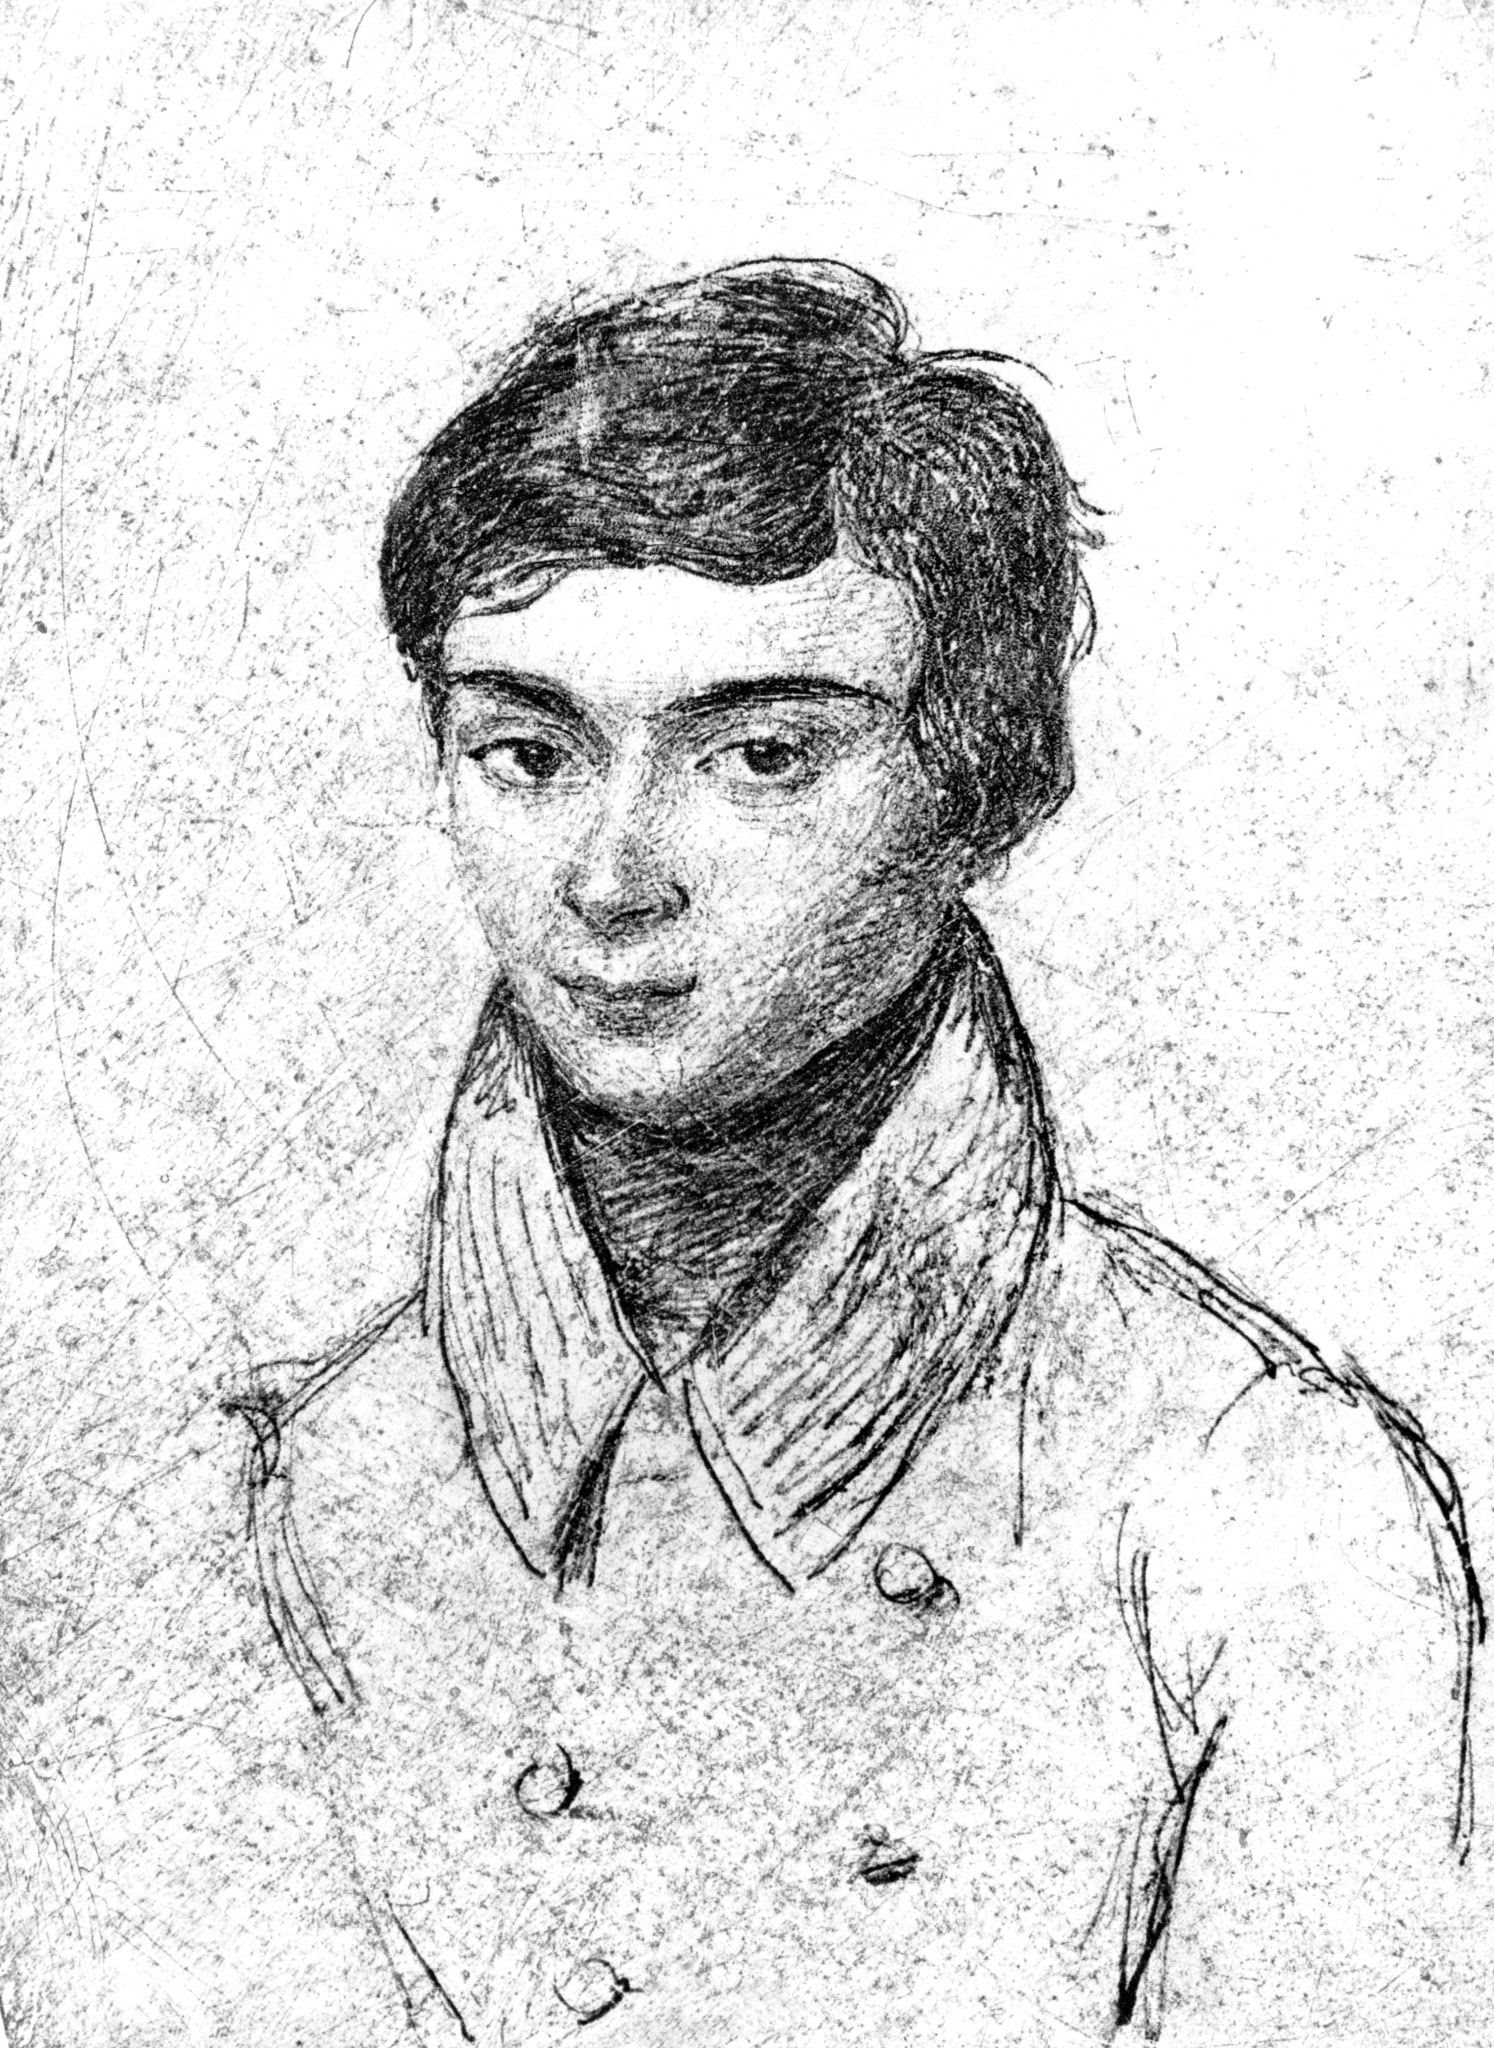
\includegraphics[width= 0.5\linewidth]{20}
%		\caption{\small\textit{\color{toanhocdoisong}Evariste Galois $(1811 - 1832)$.}}
%		\vspace*{-10pt}
%	\end{figure}
	Trong mã Reed -- Solomon, việc mã hóa được tiến hành cho từng gói gồm $k$ phần tử của $GF(2^n)$. Nói cách khác, quá trình mã hóa được tiến hành cùng lúc cho $k$ số nhị phân, mỗi số $n$ bit. Ký hiệu các phần tử của gói là $m_0,m_1,\ldots,m_{k-1}$. Ta xây dựng được một đa thức:
	\begin{align*}
		P(x)=m_0+m_1x+ \cdots +m_{k-1} x^{k-1}.
	\end{align*}
	Chú ý rằng đa thức này khác với những đa thức đã nói ở trên. Những đa thức ở phía trên có hệ số là $0$ hoặc $1$ (phần tử của $GF(2)$) còn đa thức $P(x)$ của ta có các hệ số $m_i$ là các phần tử của $GF(2^n)$. Một codeword được tạo ra bằng cách tính các giá trị của $P(x)$ cho từng phần tử của trường Galois $GF(2^n)$:
	\begin{align*}
	c &\!=\! \left(c_0,c_1,c_2,\ldots,c_{q-1}\right) \\[-0.5ex]
	&\!=\!\! \left[\!P(0), P(\!\alpha\!), P(\alpha^2), \ldots, P(\alpha^{q-1}\!)\!\right]\!,q \!=\! 2^n,
	\end{align*}
	Do mỗi phần tử $m_i$ có thể nhận một trong $q=2^n$ giá trị nên có tổng cộng $q^k$ codeword trong mã Reed -- Solomon. Ứng với mỗi codeword, ta có một hệ phương trình:
	\begin{align*}
		P(0)=\,&m_0, \\[-0.5ex]
		P(\alpha)=\,&m_0+m_1 \alpha+m_2 \alpha^2+\cdots\\[-0.5ex]
		&+m_{k-1} \alpha^{k-1},
		\end{align*}
		\begin{align*}
		P(\alpha^2 )=\,&m_0+m_1 \alpha^2+m_2 \alpha^4+\cdots\\[-0.5ex]
		&+m_{k-1} \alpha^{2(k-1)},\\[-0.5ex]
		...&\\[-0.5ex]
		P(\alpha^{q-1})=\,&m_0+m_1 \alpha^{q-1}+m_2 \alpha^{2(q-1)} \\[-0.5ex]
		&+\cdots+m_{k-1} \alpha^{(k-1)(q-1)}. 
	\end{align*}
	Chọn bất kỳ $k$ trong số $q$ phương trình trên, ta được một hệ phương trình mà từ đó có thể giải để tìm các $m_i$.
	\vskip 0.05cm
	Trong trường hợp đường truyền bị lỗi, giả sử có $t$ trong số $q$ phương trình bị lỗi (giá trị $P\left(\alpha^i\right)$ tương ứng bị lỗi). Khi đó, nếu ta thử tất cả các tổ hợp có thể gồm $k$ phương trình từ $q$ phương trình, sẽ có $( \begin{array}{l}
		t + k - 1\\[-0.5ex]
		k
	\end{array})$ hệ phương trình cho kết quả $m_i$ khác với các hệ phương trình còn lại. Do đó, việc sửa lỗi có thể được tiến hành bằng cách lấy kết quả chiếm đa số, với điều kiện là  $( \begin{array}{l}
	t + k - 1\\[-0.5ex]
	k
\end{array}) <( \begin{array}{l}
q - t\\[-0.5ex]
k
\end{array})$. Số lỗi lớn nhất có thể sửa là số nguyên $t$ nhỏ hơn hoặc bằng $\dfrac{1}{2}(q-k+1)$.
\vskip 0.05cm
	Việc thử các tổ hợp hệ phương trình khác nhau theo đề xuất ban đầu của Reed và Solomon là tương đối phức tạp về mặt cài đặt trong thực tế nên sau đó người ta đã đưa ra hai hướng tiếp cận khác để tạo mã Reed -- Solomon, một sử dụng đa thức sinh và một sử dụng biến đổi Fourier trên trường Galois (Wicker, $1994$).
	\vskip 0.05cm
	\textbf{\color{toanhocdoisong}Tài liệu tham khảo}
	\vskip 0.05cm
	[$1$] Aktaş, C. ($2017$). \textit{The evolution and emergence of QR codes}. Cambridge Scholars Publishing.
	\vskip 0.05cm
	[$2$] Reed, I. S., \& Solomon, G. ($1960$). \textit{Polynomial Codes Over Certain Finite Fields}. Journal of the Society for Industrial and Applied Mathematics, $8(2)$, $300-304$. 
	\vskip 0.05cm
	[$3$] Wicker, S. B., \& Bhargava, V. K. ($1994$). \textit{Reed--Solomon codes and their applications}. IEEE.
\end{multicols}